
            CLAS12 runs with "open trigger", which means different sub-experiments can define their own triggering logic. There is a standard electron trigger, based off of hits in HTCC, ECal, and FTOF. 

        Only about 50\% of the electron triggers recorded with an inbending torus polarity are actually electrons. For outbending torus polarity, hte electron trigger purity is as high at 70\%. 
    
    \href{https://www.jlab.org/Hall-B/clas12-web/}{Detector Specs}
    
    20 kHz Level 1 trigger rate, 1 GB/s.


    
    
            \begin{figure}[H]
    			\centering
    			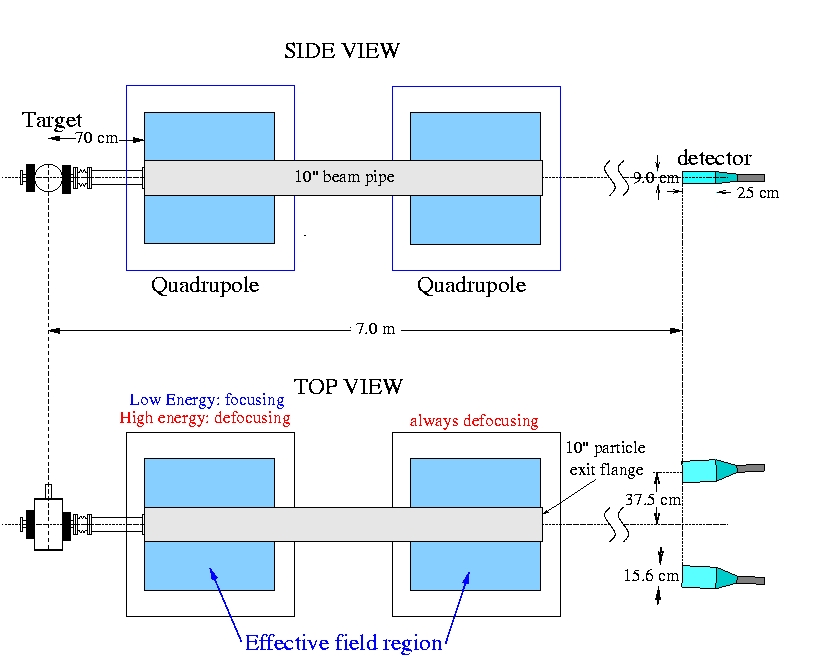
\includegraphics[width=12cm]{Chapters/Ch2-Experiment/clas-12-system/pics/other/hall-b-poll-1.jpg}
    			\caption{ }
			\end{figure}
			
												
			 \begin{figure}[H]
    			\centering
    			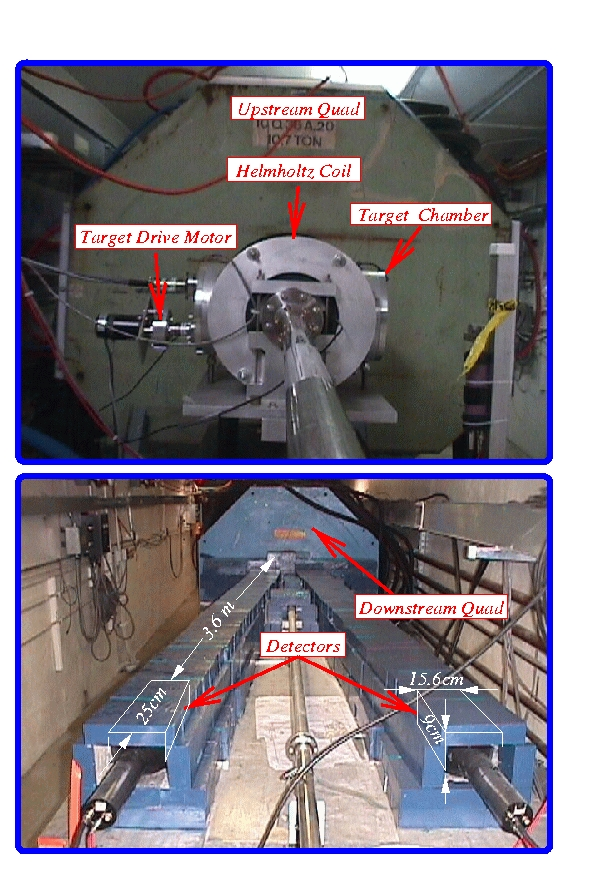
\includegraphics[width=12cm]{Chapters/Ch2-Experiment/clas-12-system/pics/other/hall-b-poll-2.jpg}
    			\caption{ }
			\end{figure}
			
			 \begin{figure}[H]
    			\centering
    			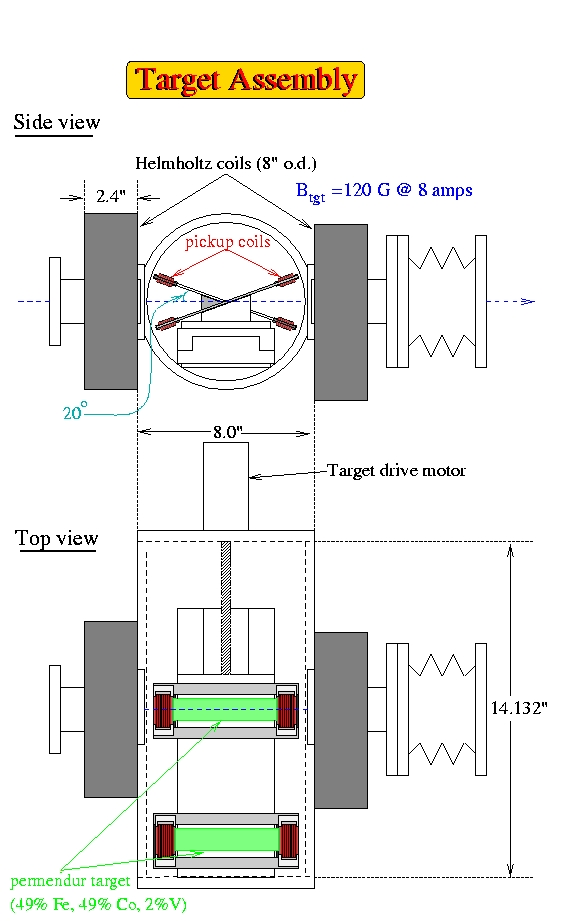
\includegraphics[width=12cm]{Chapters/Ch2-Experiment/clas-12-system/pics/other/hall-b-poll-target.jpg}
    			\caption{ }
			\end{figure}

        Data taken is RGA taken in Fall 2018